\subsection{UC3 - Gestione dei trasferimenti}
\begin{figure}[H]
    \centering
    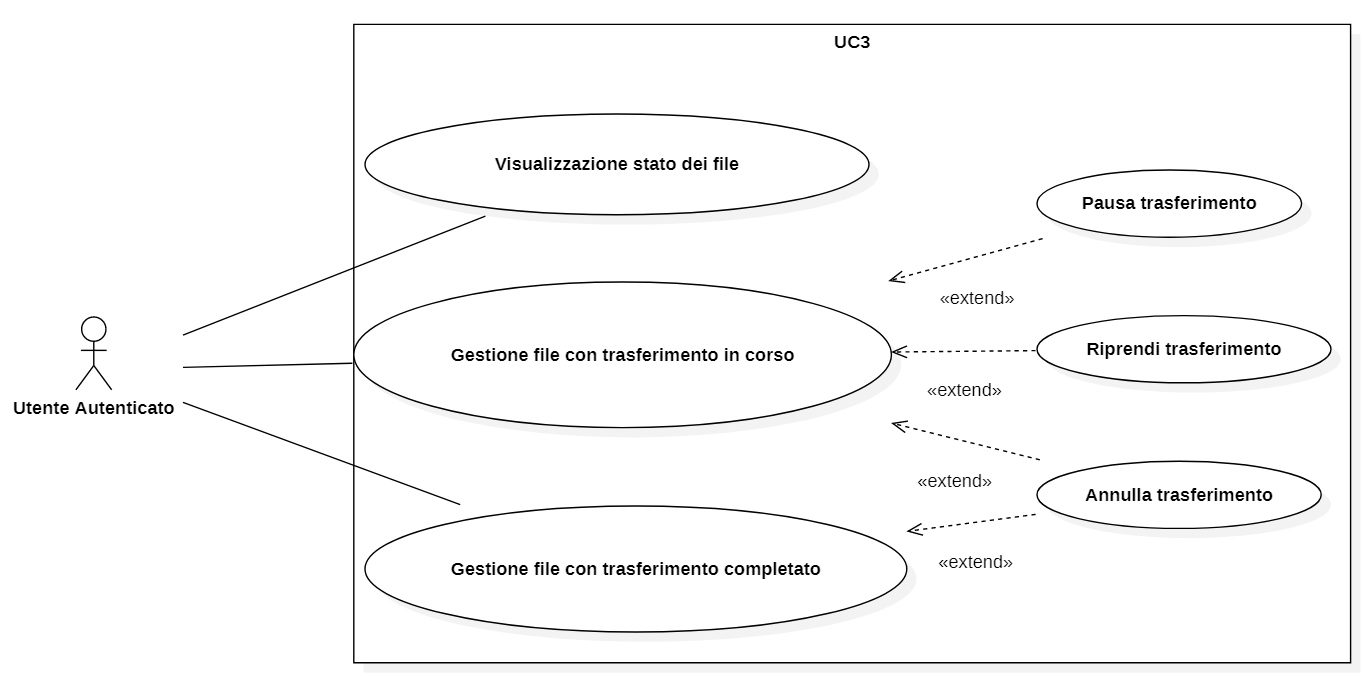
\includegraphics[scale = 0.4]{components/img/UC3.png}
    \caption{UC3 - Gestione dei trasferimenti}
\end{figure}
\begin{itemize}
\item \textbf{Attore Primario:} Utente autenticato;
\item \textbf{Precondizione:} L'utente ha a disposizione varie funzionalità per la gestione dei trasferimenti;
\item \textbf{Postcondizione:} Viene eseguita l'operazione richiesta dall'utente;
\item \textbf{Scenario principale:}
    \begin{enumerate}
    \item L'utente può visualizzare l'elenco dei file presenti nei trasferimenti ed il loro stato;
    \item L'utente può gestire i file con trasferimento in corso;
    \item L'utente può gestire i file con trasferimento completato.
    \end{enumerate}
\item \textbf{Estensioni:}
\begin{itemize}
\item L'utente può mettere in pausa un trasferimento in corso;
\item L'utete può riprendere un trasferimento in pausa;
\item L'utente può annullare un trasferimento in corso;
\item L'utente può annullare un trasferimento che è stato completato.
\end{itemize}
\end{itemize}